\documentclass[a4paper, oneside]{memoir}
\usepackage[utf8]{inputenc}
%\usepackage[T1]{fontenc}
\usepackage{verbatim}
\usepackage{graphicx}
\usepackage{listings}
\usepackage{listing}
\usepackage{amsthm}
\usepackage{amsfonts}
\usepackage{amsmath}
\usepackage{subfig}
\usepackage{varioref}
\usepackage{color}
\usepackage{pgf}
\usepackage[colorinlistoftodos]{todonotes}
%\usepackage[colorlinks, linkcolor=blue, citecolor=red, urlcolor=brown]{hyperref}
\usepackage{hyperref}
% ^- farver gør det meget nederen at udskrive en s/h kopi, da alle "se
% fig 1.1 på side xx" bliver grå! (ptx)

\usepackage{natbib}

%Individual todos
\newcommand{\todoPtx}[2][]{\todo[color=red,    #1]{Ptx: #2}}
\newcommand{\todoCpvc}[2][]{\todo[color=yellow, #1]{Cpvc: #2}}
\newcommand{\todoSean}[2][]{\todo[color=pink,   #1]{Sean: #2}}
\newcommand{\todoHave}[2][]{\todo[color=green,  #1]{Have: #2}}
\newcommand{\todoVester}[2][]{\todo[color=blue,  #1]{Vester: #2}}

\renewcommand{\ttdefault}{pcr}


\lstset{language=C}
%\lstset{backgroundcolor=listinggray}
%\lstset{backgroundcolor=\color{listinggray}}
%\lstset{linewidth=90mm}
%\lstset{frameround=tttt}
%\lstset{frameround=trbl}
%\lstset{labelstep=1}
%\lstset{keywordstyle=\color{blue}\textbf}
\lstset{keywordstyle=\textbf}
%\lstset{moredelim=[is][\ttfamily]{|}{|}}
\lstset{basicstyle=\ttfamily \footnotesize}
%\lstset{basicstyle=\ttfamily \small}
\lstset{commentstyle=\ttfamily}
\lstset{stringstyle=\bfseries}
\lstset{showstringspaces=false}
%\lstset{numbers=left,numberstyle=\ttfamily \small}
%\lstset{breaklines=true}


% \lstset{
%   basicstyle=\ttfamily \footnotesize,
%   keywordstyle=\color{red}
% }


% Dokumantation:
% http://www.tex.ac.uk/tex-archive/macros/latex/contrib/todonotes/todonotes.pdf
% Vigtigste kommandoer:
% \todoVester[inline]{text}
% \missingfigure{A illustration of how peers are placed on the ring}
% \todo{Introduction to this section}
% \todo[inline]{Someone write this}

% replaces cite. Use \cit instead!
\newcommand{\cit}[1] {\cite{#1}}

% cite with page or section ref
\newcommand{\citbook}[2] {\citep[#2]{#1}}

% when defining a new term
\newcommand{\dit}[1] {\textit{#1}}

% \image{image, scale, caption, label}
\newcommand{\image}[4]{
  \begin{figure*}[!htb]
    \centering
    \includegraphics[scale=#2]{imgs/#1}
    \caption{#3}
    \label{#4}
  \end{figure*}}
% ^- Det her går aldrig godt, man har aldrig brug for at ændre flere
% ting end der er muligt med denne slags makroer. (ptx)

\title{Level Sets!!}
\author{
 \\
  Martin Have (2005????)\\
  \url{have@cs.au.dk}\\
  \\
  Peter Kristensen (20051866)\\
  \url{ptx@cs.au.dk}\\
  \\
  Mikkel Vester (20053229)\\
  \url{vester@cs.au.dk}\\
  \\
  Cpvc (200?????)\\
  \url{cpvc@cs.au.dk}\\
  \\
  Hitler (Moralsk support)\\
  \url{hitler@cs.au.dk}\\
  \\
  University of Aarhus
}

\begin{document}

\maketitle{}


\missingfigure{Her er et billede af et morph ting}

% Hvem laver hvad.
\begin{comment} % orgtbl-mode er win
|----------------------------+----------+--------|
| Afsnit                     | Indhold  | Hvem   |
|----------------------------+----------+--------|
| Intro                      | ch. 1,2  | have   |
| Build SDF / Discretization | artikel? | vester |
| Reinitialize               | ch. 7    | cpvc   |
| Motion                     | ch. 4,6  | ptx    |
| Externally gen. vf.        | ch. 3    | geggie |
| Godunov                    | ch. 5    | cpvc   |
|----------------------------+----------+--------|
\end{comment}

\newpage

\tableofcontents{}
\listoftodos
\chapter{Introduction}
\label{chap:introduction}
  In this report, we will explain what the Level Set method is and what
its applications are. Furthermore, we will provide code examples of
how to implement the mathematical formulas needed to create a Level
Set framework.

The Level Set method is a numerical technique used to transform
surfaces in $d$ dimensions. Transform means that we move the surface. The surfaces are transformed by solving a
partial differential equation(PDE) dependant on a time factor.

The level set at its most simple representation is a static
datastructure. It can be represented as a topographic map indicating
heights in a region, displayed in figure \vref{fig:isocontour-2d} or
it can be seen as a meteorological map, displaying weather data like
pressure. 
In figure \vref{fig:heightmap} we see two figures describing a 2-d and 3-d view of an island. Figure \vref{fig:isocontour-2d} describes an isocontour map of heights where the color indicates the height of each point. The brighter the color the higher the point. Figure \vref{fig:isocontour-3d} shows the corresponding 3d view.  

\begin{figure}[h]
\begin{center}
  \subfloat[2D view of an elevation isocontour map]{
    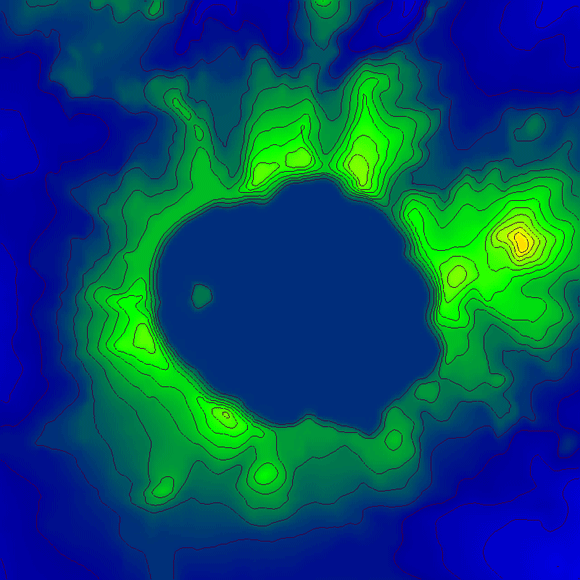
\includegraphics[width=0.5\textwidth]{imgs/226171_226171.png}
    \label{fig:isocontour-2d}
  }
  \subfloat[3D view of figure \ref{fig:isocontour-2d}]{
    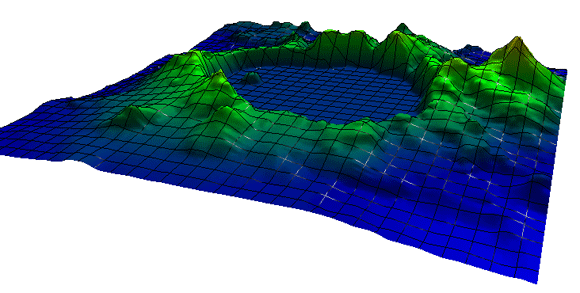
\includegraphics[width=0.5\textwidth]{imgs/226170_226170.png}
    \label{fig:isocontour-3d}
  }
\end{center}
\caption{Illustrations of heightmap, from: Intel Array Visualizer Gallery}
\label{fig:heightmap}
\end{figure}

%Intel Array Visualizer Gallery
%website\footnote{\url{http://www.intel.com/cd/software/products/apac/zho/perflib/226296.htm}}
\todoHave{husk reference}

%\image{hoejdekort.png}{0.25}{A topographic map indicating heights in the vermont region.}{introduction:fig:hoejdekort}

\section*{Signed distance function - $\phi$}

We would like a suitable way to indicate whether we are inside or outside the isocontour. 

We use an implicit representation of the surface. The Level Set method
can use implicit functions which means that the function is defined in
the entire plane and not only on the object.

The function $\phi(x,y)$ is a signed distance function in all of
$\mathbb{R}^{n}$, in our case $\mathbb{R}^{2}$. A signed distance
function $\phi$ is a function that given a point on the plane, returns
the distance to the surface. We have that $\phi(x,y) > 0$ if we are
outside the object and $\phi(x,y) < 0$ when we are inside the object.
And last, when $\phi(x,y) = 0$ we are on the interface or iso-surface.
The iso-surface separates the inside and outside.  Besides indicating
whether we are inside or outside an object, it also indicates how far
we are from the closest point on the iso-surface which is quite
handy. For a picture of the above, see figure
\vref{introduction:fig:implicitfunction}.

\image{phi.png}{0.3}{The figure is borrowed from
\cit{osher2002level}. A implicit function, defined in all of
$\mathbb{R}^{2}$. We see that when we are inside the object then
$\phi$ is less than zero, larger when we are outside and zero on the
interface.}{introduction:fig:implicitfunction}

%% Example - Circle

\subsection*{Example}

A simple example is to consider a circle and its equation:
\begin{equation*} 
  x^{2} + y^{2} = r^{2}
\end{equation*}

It is defined in all points in $\mathbb{R}^{2}$ and is an example of
an implicit function. Given a specific radius $r$, the equation of a
circle defines an isocontour. If $r = 5$, then the isovalue is $c =
5^{2} = 25$. For all the points $(x,y)$ that evaluate to 25 gives us
the isosurface. If the value is smaller then it is inside the surface,
and outside when the value is greater. See figure
\vref{introduction:fig:cartesiangrid}.


\section*{Cartesian grid}
\begin{comment} Finite memory -> descritization of plane -> cartesian
grid is used.
\end{comment}

Since a computer has finite memory we need to come up with a way to
store our representation. A simple way to do this that scale in the
number of dimensions is to partition the region into a grid where each
square is of equal size.

\begin{figure}[htb] \centering
    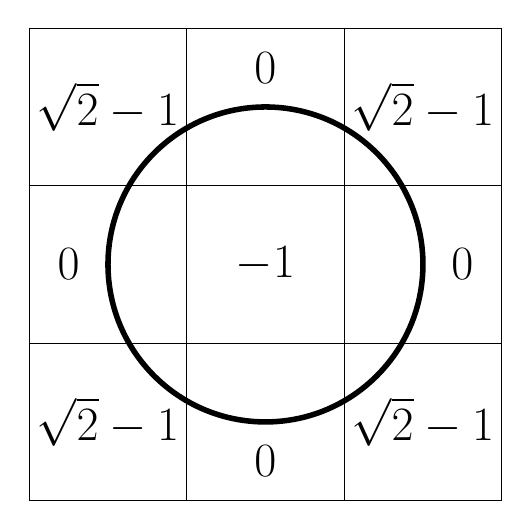
\begin{tikzpicture}[font=\LARGE]
    \draw (0,0) rectangle +(2,2)
    +(1,1) node {$-1$};
    \draw (0,2) rectangle +(2,2)
    +(1,1.5) node {$0$};
    \draw (2,0) rectangle +(2,2)
    +(1.5,1) node {$0$};
    \draw (0,-2) rectangle +(2,2)
    +(1,0.5) node {$0$};
    \draw (-2,0) rectangle +(2,2)
    +(0.5,1) node {$0$};
    \draw (2,2) rectangle +(2,2)
    +(1,1) node {$\sqrt{2}-1$};
    \draw (2,-2) rectangle +(2,2)
    +(1,1) node {$\sqrt{2}-1$};
    \draw (-2,2) rectangle +(2,2)
    +(1,1) node {$\sqrt{2}-1$};
    \draw (-2,-2) rectangle +(2,2)
    +(1,1) node {$\sqrt{2}-1$};
    \draw[line width=2pt] (1,1) circle (2);
  \end{tikzpicture}
  \caption{Borrowed from \cit{JLTGK}. A circle, descritized into a
cartesian grid. The value in each cell is the $\phi$ value described
in this chapter.}
  \label{introduction:fig:cartesiangrid}
\end{figure}

In figure \vref{introduction:fig:cartesiangrid}, we see how a plane
has been descritized into a cartesian grid, showing a circle and the
values of $\phi$.

%% formulas

\section*{Solving the Level Set}\label{sec:intro:solve} 

\todoPtx{I own this!!}

If we want to move the level set, we have to iteratively solve a Partial
differential equation to make the surface move. We solve a partial
differential equation in all points $(x,y) | x,y \in
\mathbb{R}^{2}$. If we want to move the interface in the normal
direction we solve the following equation:

\begin{equation}
\phi_{t} + a|\nabla \phi| = 0
\end{equation}\label{eq:normMove}

where $\nabla \phi = (\dfrac{\partial \phi}{\partial x},
\dfrac{\partial \phi}{\partial y})$ and $a$ can be of either sign.

When $a > 0$ the interface moves in the normal direction and when $a <
0$ it moves in the opposite direction of the normal.


\section*{Applications}

The advantages are that since we discretize the surface into a
cartesian grid, we can do numerical computations without having to
parameterize the objects. Another advantage is that the level set
method makes it easy to work on geometry that change topology over
time.


%% applications.  So why do we want to use the level set method? A
simple example is to consider an object that splits in two or two
objects merging into one. If we did not use the level set method, we
would have to explicitely represent the two new objects, where in the
level set case we get this for free do to the implicit representation.

\todoPtx{måske lidt flere anvendelsesmuligheder (lysberegninger her!)}

\newpage

\section*{Outline of the report}\todoPtx{Denne er på en side for sige
selv, så vref ikke crasher}

In chapter \vref{chap:sdf}, we give an in depth look on the signed
distance function, describe what kinds of mathematical operations we
have in our toolbox and describe the important reinitialize function,
section \vref{sec:reinitialize}.

In chapter \vref{chap:extensions}, we look at extension that can be
made to the basic level set implementation that we have done. In
section \vref{sec:segmentation}, we look at how to implement
segmentation algorithms which can be used in mediacal imaging. In
section \vref{sec:fluid}, we implement a fluid solver for computer
graphics using the level set method. And finally, in section
\vref{sec:imagereconstruction} \todoHave{Skal CPVC's afsnit være med i
den endelige rapport? (have)} we use the level set to do computations
on images.



%%% Local Variables: 
%%% mode: latex 
%%% mode: auto-fill 
%%% TeX-PDF-mode: t 
%%% TeX-master: "../master.tex" 
%%% End:



\chapter{SDF}
\label{chap:sdf}
\todoVester{tekst her}

\section{Mikkel-Sean Algorithm TM}
\label{sec:initialization}
\todo{Dette er et eksempel på en todo for alle}

\pagebreak
\section{Reinitialization}
\label{sec:reinitialize}
% -*- mode: latex; mode: auto-fill; coding: utf-8; -*-

The main advantage of representing an implicit counture or surface as
a signed distance field, is that the length of the gradient is
one. This is also exactly what defines a signed distance field.

When constructing or manipulating a signed distance field defined on a
Cartesean grid, the result is not always signed distance field. So to
enable further calculations or iterations of an algorithm the result
must be turned into a new signed distance field that reflexts the
changes done by the calculations. This process is called
\dit{reinitialization} of the level set, and can be done several
different ways.

Algorithms to reinitializing signed distance fields focuses on
reinitializing the whole domain, and at the same time keeping the zero
level set as fixed as possible. This means that the process disrupts
data outside the zero level set, which depending on the type of
phemomena we are modelling can be problematic. For the problems we are
modelling this is not an issue, and is therefore not of relevance here.

Before diving into the algoritms a good question is, how often must the
level set be reinitialized? There is no good answer to this question,
because it depends on how rapidly the contour is changing. In our work
we have been reinitializing after ever change, which ensures that this
is not a source of error.

The two most used algoritmic approched to reinitialization are:
geometricly methods that calculations distances to the contour or surface,
and PDE based methods that numerical approximates solutions to the Eikonal
equation: $||\nabla \phi|| = 1$ \citbook{book:fluids}{page~89}.

When initializing the implicit contour in section \vref{sec:initialization}
we used an algorithm that geometricly calculated the distance to the
contour. So the natural choise should be also to use this algorithm for
reinitializing, but because the algorithm does not calculate the
signed distance function precise enough, we cannot use this algorithm
when reinitializing. Furthermore if we had used this type of
algorithm, the we would have had to construct the contour before
invoking the algorithm. Constructing the contour is very expensive,
and is something that should be avoided at almost all cost when using
the level set method.

Instead we have chosen to use PDEs to solve the Eikonal
equation. Solving the Eikonal equation can also be done in different
ways, which we will describe in the next subsections.

\subsection{The PDE way of reinintalizing}
When using the PDE way of reinitialing the level set, we solve the
following PDE \citbook{book:levelset}{page~65-66}:

\begin{equation}
\label{eq:reinit}
\phi_t + S(\phi_0)(|\nabla \phi| - 1) = 0
\end{equation}

Where $\phi$ is the SDF being evolved as a PDE, and $\phi_0$, is the
initial SDF giving as input to the reinitialization algorithm, which
has not been altered by the process of solving the PDE. The function
$S(\phi_0)$ gives the sign of the SDF, like the following function,
described in \citbook{book:LS}{page~66}:
%\citbook{article:FLLSM}{page~419}:

\begin{equation}
\label{eq:s1}
S(\phi) =
\begin{cases}
-1 &\mbox{ if } \phi < 0, \\
 0 &\mbox{ if } \phi = 0, \\
 1 &\mbox{ if } \phi > 0.
\end{cases}
\end{equation}

When using this approach of reinitializing the SDF, then the grid
points in $\phi$ that are nearest to the contour is reinitialized
first, and then propergated in the normal direction from the zero
level set, hereby reinitializing the grids points in layers each
iteration.

This algorithm is relatively slow if all grid points needs to be
reinitialized, because it only reinitializes one layer in each
iteration when solving the PDE. This means that the PDE, on a
two-dimensional domain, must be iterated
$\sqrt{width^2 \times height^2}$ times to make sure that the algoritm
has reinitialized the whole domain.

But because the algorithm has the property of reinitializing the SDF
in layers it is of special interest in reguards to performance when
using a narrow band level set as described in section
\vref{sec:band}. Here only three or four layers around the SDF needs
to be reinitialized, making the algorithm ideal for the narrow band
approach.

\subsection{The sign function S}
Because equation \ref{eq:reinit} is a hyperbolic PDE, we need to use a
smeared out version of equation \eqref{eq:s1}. One way of smearing the
function is to using equation \eqref{eq:Sphi0}.

\begin{equation}
\label{eq:Sphi0}
S(\phi_0) = \frac{\phi_0}{\sqrt{\phi_0^2 + (\Delta x)^2}}
\end{equation}

The difference between equation \eqref{eq:s1} and equation
\eqref{eq:Sphi0}, can more easily be seen be looking at a plot of the
two functions, as depicted in figure \ref{fig:s-graph}.

\begin{figure}[h]
\begin{center}
  \subfloat[Plot of equation \eqref{eq:s1}]{
    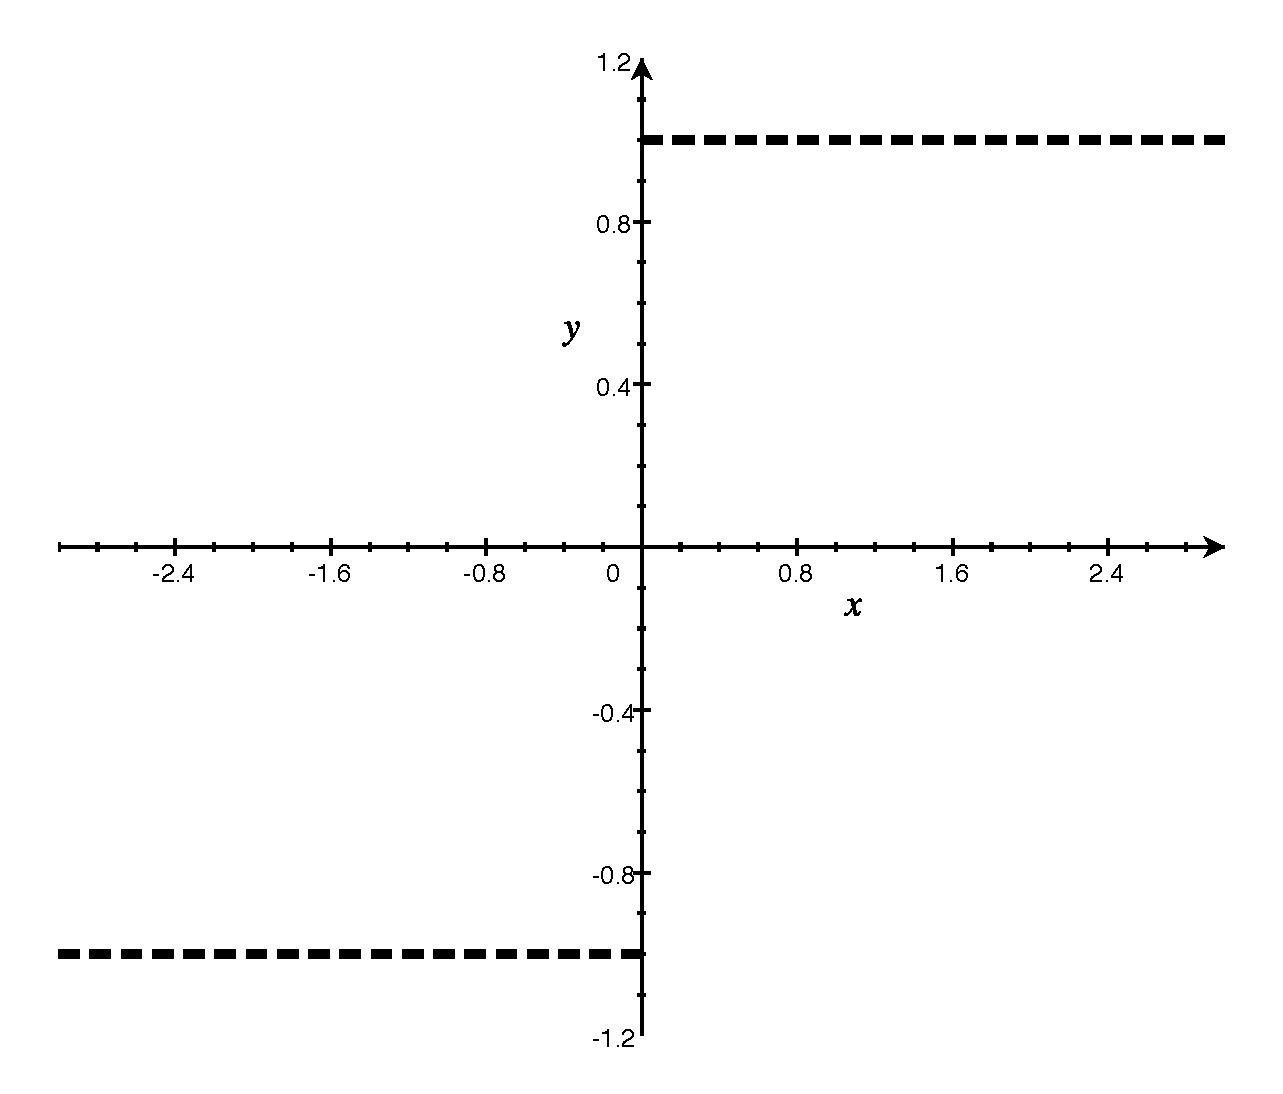
\includegraphics[width=0.5\textwidth]{imgs/S0.pdf}
    \label{fig:fake1}
  }
  \subfloat[Plot of equation \eqref{eq:Sphi0}, $\Delta x=1$]{
    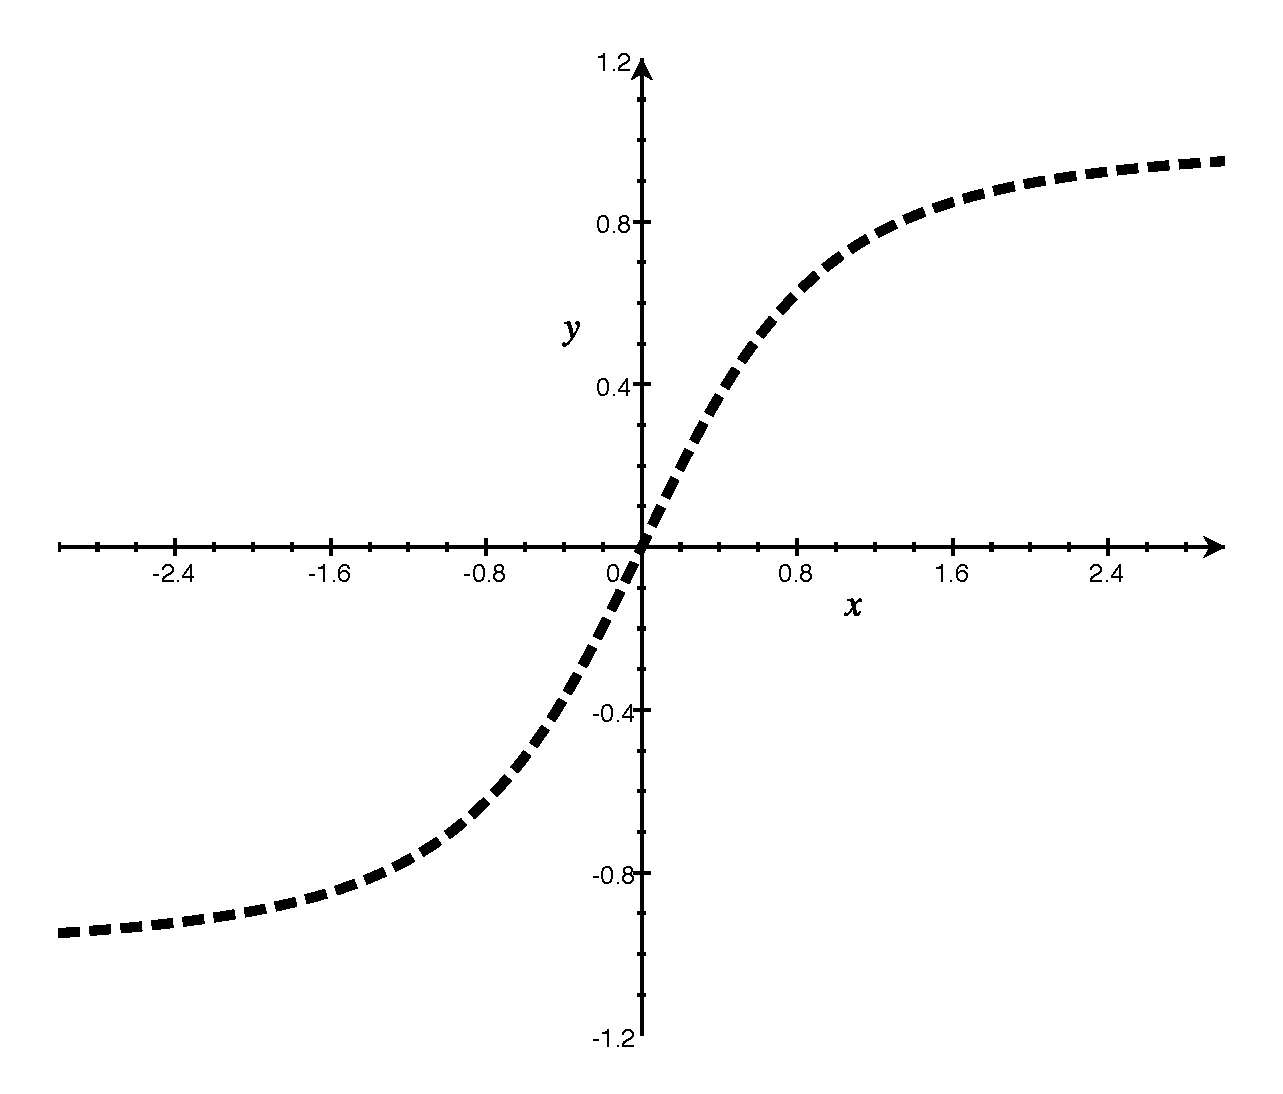
\includegraphics[width=0.5\textwidth]{imgs/S1.pdf}
    \label{fig:fake2}
  }
\end{center}
\caption{Illustrations of S}
\label{fig:s-graph}
\end{figure}

%\subsection{CFL-condition}


\pagebreak
\subsection{Implementation}
The implementation of how to solve the PDE from equation \eqref{},
uses the describtion Godunov's scheme from \citbook{book:LS}{page~58}
in the spatial dimensions, and a forward Euler in time, described in
formular (1.3) in \citbook{book:LS}{page~10}.

\begin{lstlisting}[language=c++]
    Tex<float> phi0 = GetPhi(); Tex<float> phin = GetPhi();
    for (unsigned int i = 0; i<iterations; i++) {
        for (unsigned int x = 0; x < width; x++) {
            for (unsigned int y = 0; y < height; y++) {
                float xy = phi(x, y);                
                float phiXPlus = 0.0f;
                float phiXMinus = 0.0f;
                float phiYPlus = 0.0f;
                float phiYMinus = 0.0f;        	
                if (x != width-1) phiXPlus  = (phi(x+1, y) - xy);
                if (x != 0)       phiXMinus = (xy - phi(x-1, y));
                if (y !=height-1) phiYPlus  = (phi(x, y+1) - xy);
                if (y != 0)       phiYMinus = (xy - phi(x, y-1));
        	
                float dXSquared = 0;
                float dYSquared = 0;
                float a = phi0(x,y);
                if (a > 0) {
                    // formula 6.3 page 58
                    float max = std::max(phiXMinus, 0.0f);
                    float min = std::min(phiXPlus, 0.0f);
                    dXSquared = std::max(max*max, min*min);
                    max = std::max(phiYMinus, 0.0f);
                    min = std::min(phiYPlus, 0.0f);
                    dYSquared = std::max(max*max, min*min);
                } else {
                    // formula 6.4 page 58
                    float max = std::max(phiXPlus, 0.0f);
                    float min = std::min(phiXMinus, 0.0f);
                    dXSquared = std::max(max*max, min*min);
                    max = std::max(phiYPlus, 0.0f);
                    min = std::min(phiYMinus, 0.0f);
                    dYSquared = std::max(max*max, min*min);        				
                }
                float normSquared = dXSquared + dYSquared;           
                float norm = sqrt(normSquared);

                // Using the S(phi) sign formula 7.6 on page 67
                float sign = phi0(x,y) / sqrt(phi0(x,y)*phi0(x,y) + 1);
                float dt = 0.3; // A stabil CFL condition
                phin(x,y) = phi(x,y) - sign*(norm - 1)*dt;
            }
        }
        for (unsigned int y=0; y<height ; y++)
            for (unsigned int x=0; x<width; x++)
                phi(x,y) = phin(x,y);

    }
\end{lstlisting}


\section{CSG (Union, Intersetion, Minus)}
\subsection{Union}
\subsection{Intersetion}
\subsection{Minus}

\section{Motion (grow/shrink, mean-curvature, morph, CFG condition)}
\subsection{Grow/Shrink}

\todoPtx{Grow/shrink!}

%%% Local Variables: 
%%% mode: latex
%%% TeX-master: "../../master"
%%% End: 

\subsection{Mean-Curvature}

\todoPtx{Mean-Curvature}

%%% Local Variables: 
%%% mode: latex
%%% TeX-master: "../../master"
%%% End: 

\subsection{Morph}

\todoPtx{Morph}

%%% Local Variables: 
%%% mode: latex
%%% TeX-master: "../../master"
%%% End: 

\subsection{CFG condition (Stability)}

\todoPtx{CFG}

%%% Local Variables: 
%%% mode: latex
%%% TeX-master: "../../master"
%%% End: 


\chapter{Extensions}
\label{chap:extensions}

\section{Narrow-band}
\label{sec:narrowband}
\todoVester{skriv om narrow band}

\section{3D}
\label{sec:3d}

\section{CUDA}
\label{sec:cuda}

Improving the performance of our algorithms can be done in many ways,
but one of the more obvious ones are using parallel computing!

Currently, the most accessible way to run programs in parallel is
using the graphics computation unit (GPU). Modern GPUs are very
powerful, and major manufactures have released software development
kits (SDK) for utilise the GPU for general purpose computation.

One of these SDKs is nVidias CUDA\cit{cuda}. The only thing needed to
use CUDA is a nvidia graphics card that is relatively new (a few years
tops), and the free SDK found at the CUDA website.

As GPUs were developed to render graphics, they are optimized to work
on spatially coherent data. This makes many of our algorithms a
natural target, as we often only need information about neighbouring
data points.

% section?
\subsection{Memory?}

When a algorithm have been implemented using CUDA, there are many ways
to optimize it. Often memory access is the biggest problem.

Because of the architecture of GPUs, CUDA have many different types of
memory. Each with different properties and uses.

\todoPtx{Skriv om threads?}

% code

\begin{lstlisting}
#define GetPhi(phi,x,y,w) phi[x+w*(y)]

void cu_Init() {}


__global__ void reinit(float *phi,float* phi0, float* phin, 
                       unsigned int width, unsigned int height) {
    uint x = __umul24(blockIdx.x, blockDim.x) + threadIdx.x;
    uint y = __umul24(blockIdx.y, blockDim.y) + threadIdx.y;

    if (x > width || y > height)
        return;
    
    float xy = GetPhi(phi,x,y,width);

    float phiXPlus = 0.0f;
    float phiXMinus = 0.0f;
    float phiYPlus = 0.0f;
    float phiYMinus = 0.0f;        	
    if (x != width-1) phiXPlus  = (GetPhi(phi,x+1, y,width) - xy);
    if (x != 0)       phiXMinus = (xy - GetPhi(phi,x-1, y,width));
    
    if (y !=height-1) phiYPlus  = (GetPhi(phi,x, y+1,width) - xy);
    if (y != 0)       phiYMinus = (xy - GetPhi(phi,x, y-1,width));

    /* GetPhi(phin,x,y,width) = phiYPlus; */
    /* return; */


    float dXSquared = 0;
    float dYSquared = 0;
    float a = GetPhi(phi0,x,y,width);
    if (a > 0) {
        // formula 6.3 page 58
        float _max = max(phiXMinus, 0.0f);
        float _min = min(phiXPlus, 0.0f);
        dXSquared = max(_max*_max, _min*_min);
                    
        _max = max(phiYMinus, 0.0f);
        _min = min(phiYPlus, 0.0f);
        dYSquared = max(_max*_max, _min*_min);
    } else {
        // formula 6.4 page 58
        float _max = max(phiXPlus, 0.0f);
        float _min = min(phiXMinus, 0.0f);
        dXSquared = max(_max*_max, _min*_min);
                    
        _max = max(phiYPlus, 0.0f);
        _min = min(phiYMinus, 0.0f);
        dYSquared = max(_max*_max, _min*_min);        				
    }

    float normSquared = dXSquared + dYSquared;           
    float norm = sqrt(normSquared);

    // Using the S(phi) sign formula 7.6 on page 67
    //float sign = phi(x,y) / sqrt(phi(x,y)*phi(x,y) + normSquared);
    float sign = GetPhi(phi0,x,y,width) / 
        sqrt(GetPhi(phi0,x,y,width)*GetPhi(phi0,x,y,width) + 1);
    float t = 0.3; // A stabil CFL condition
    GetPhi(phin,x,y,width) = GetPhi(phi,x,y,width) - sign*(norm - 1)*t;


}

void cu_Reinit(float* data, 
               unsigned int w,
               unsigned int h,
               unsigned int iterations) {
    float* phiData;
    float* phi0Data;
    float* phinData;

    cudaMalloc((void**)&phiData, sizeof(float)*w*h);
    cudaMalloc((void**)&phi0Data, sizeof(float)*w*h);
    cudaMalloc((void**)&phinData, sizeof(float)*w*h);
    cudaMemcpy((void*)phiData,(void*)data, sizeof(float)*w*h,cudaMemcpyHostToDevice);
    cudaMemcpy((void*)phi0Data,(void*)data, sizeof(float)*w*h,cudaMemcpyHostToDevice);
    cudaMemcpy((void*)phinData,(void*)data, sizeof(float)*w*h,cudaMemcpyHostToDevice);


    CHECK_FOR_CUDA_ERROR();

    const dim3 blockSize(32,16,1);
    const dim3 gridSize(w/blockSize.x, h/blockSize.y);

    for (unsigned int i=0;i<iterations;i++) {
        reinit<<<gridSize,blockSize>>>(phiData,phi0Data,phinData,w,h);
        float* tmp = phiData;
        phiData = phinData;
        phinData = tmp;

        cudaThreadSynchronize();
        CHECK_FOR_CUDA_ERROR();
    }

    cudaMemcpy((void*)data,(void*)phiData, sizeof(float)*w*h,cudaMemcpyDeviceToHost);
    CHECK_FOR_CUDA_ERROR();
    cudaFree(phiData);
    cudaFree(phi0Data);
    cudaFree(phinData);
}

\end{lstlisting}

\todoPtx{CUDA coda}
\subsection{Results}

The results in table \ref{tbl:cudaRes} are taken from a system with a
1.8 Ghz Intel Core 2 Duo CPU, 4 GB RAM and a 512MB nVidia GeForce
9600M GT. The time is an average of about 100 iterations of the
algorithm.

\begin{table}[h]
  \centering
  \begin{tabular}{|l|r|r|r|}
    \hline    Algorithm & CPU & GPU & Speedup \\
    % BEGIN RECEIVE ORGTBL numbers
\hline
Reinitialization & 417825 usec & 136675 usec & 2.5987123 \\
- with textures & - & 100006 usec & 3.5515769 \\
\hline
    % END RECEIVE ORGTBL numbers
  \end{tabular}
  \caption{GPU vs. CPU comparison}
  \label{tbl:cudaRes}
\end{table}

The results shows a significant speedup. Using a quite
naive implementation the speedup is easily more than doubled on a inexpensive
consumer graphics card.

\todoPtx{Picture!}


% grep Reinit run1.log | grep CUDA | awk '{sum+=$7} END {print "avg=",sum/NR}'


\begin{comment}
#+ORGTBL: SEND numbers orgtbl-to-latex :splice t :skip 2
|------------------+-------------+-------------+-----------|
|                  | CPU         | GPU         |   Speedup |
|------------------+-------------+-------------+-----------|
| Reinitialization | 417825 usec | 136675 usec | 3.0570697 |
| - with textures  | -           | 100006 usec | 4.1779993 |
|------------------+-------------+-------------+-----------|
#+TBLFM: @2$4=@2$2 / @2$3::@3$4=@2$2 / @3$3
\end{comment}


%%% Local Variables: 
%%% mode: latex
%%% mode: auto-fill
%%% mode: orgtbl
%%% TeX-PDF-mode: t
%%% TeX-master: "../master.tex"
%%% End: 


\section{Segmentation}
\label{sec:segmentation}
\begin{comment}
  Martin har tænkt sig at skrive noget fornuftigt om segementering engang!
\end{comment}


\section{Fluid / Smoke}
\label{sec:fluid}

\section{Image Vision}
\label{sec:imagevision}

\appendix

\newpage


\bibliographystyle{alpha}
\bibliography{text/levelset}


\end{document}


%%% Local Variables: 
%%% mode: latex
%%% TeX-master: t
%%% End: 
